\documentclass[10pt,twocolumn,letterpaper]{article}

\usepackage{wacv}
\usepackage{times}
\usepackage{epsfig}
\usepackage{graphicx}
\usepackage[dvips]{graphicx}
\usepackage{amsmath}
\usepackage{amssymb}
\usepackage{multirow}

% Include other packages here, before hyperref.

% If you comment hyperref and then uncomment it, you should delete
% egpaper.aux before re-running latex.  (Or just hit 'q' on the first latex
% run, let it finish, and you should be clear).
%\usepackage[pagebackref=true,breaklinks=true,letterpaper=true,colorlinks,bookmarks=false]{hyperref}

%\wacvfinalcopy % *** Uncomment this line for the final submission

\def\wacvPaperID{****} % *** Enter the wacv Paper ID here
\def\httilde{\mbox{\tt\raisebox{-.5ex}{\symbol{126}}}}

% Pages are numbered in submission mode, and unnumbered in camera-ready
\ifwacvfinal\pagestyle{empty}\fi
\setcounter{page}{1}
\begin{document}

%%%%%%%%% TITLE
\title{Instance Segmentation of Deep Sea Scaleworms at Hydrothermal Vent}

% Authors at the same institution
%\author{First Author \hspace{2cm} Second Author \\
%Institution1\\
%{\tt\small firstauthor@i1.org}
%}
% Authors at different institutions
\author{First Author \\
Institution1\\
{\tt\small firstauthor@i1.org}
\and
Second Author \\
Institution2\\
{\tt\small secondauthor@i2.org}
}

\maketitle
\ifwacvfinal\thispagestyle{empty}\fi

%%%%%%%%% ABSTRACT
\begin{abstract}
   #TODO: Written at the end.
\end{abstract}

%%%%%%%%% BODY TEXT
\section{Introduction}

- OOI motivation, NSF goals etc. Cabled array setup in ocean. Observe and Explore deep sea (depth) and hydrothermal vent. probably an image to show where it is located. Mushroom, the hydrothermal vent being observed.

- CamHD instrument. Videos spanning the Mushroom, different zoom levels, taken continuously over years. Capturing colorful diverse benthic biology site. Extreme environment - temp (different between head (freezing) and toe (burning)), pressure, toxins, no sunlight. But due to Chemosynthesis: life is thriving, thanks to bacteria. Many organisms live in this area - examples like tubeworms, arachnids, starfishes, crabs, scaleworms and many more unidentified species. Underwater robots helped in discovering these species, and such short-term video surveillances were mostly manually analyzed to study these species. We need long-term population studies can unravel many mysteries of this world and help us in understanding how to conserve such environments. But it was hard to study these areas due to their challenging locations. But, with video data from CamHD (which we have open-sourced for research purposes), we have means to perform long-term studies this region, but manually not possible because of the volume of data. Therefore, automatic analysis is required.

- In this paper, we consider one such species found in these videos - Scaleworms, which have been biologically studied and found to have interesting properties as found in the Nature article \href{Nature article}{https://www.nature.com/articles/srep46205}, and from \href{another study}{https://pdfs.semanticscholar.org/49ae/4831505b891f771d468bcd9f5df8ca3caf92.pdf}. We propose an application of an instance segmentation method to identify, count and estimate the size of each scaleworm from a video frame. We believe that such a system will help in opening up the possibilities for large-scale population studies on such species, which currently is not available as fr as we know.

- Challenge: We discuss various challenges in analysing this data. Video, non-constant static regions, schliren distortions, lighting failures, and the nature of our target object - scale worms. The scaleworms vary in size, color shades and often look camafloughed due to the dense surrounding having dynamic colors. Also, they often stay on plant-like tube worms which keep oscillating at times due to the force of the fumes coming out of the vent. And the shortage of labeled data.

<a frame image where scaleworms are marked in green arrow marks and confusing objects are marked with red arrow marks and labeled to give reader an idea of the image we are dealing with>

Paper organization: lit-survey, problem statement, methodology, results with discussions and limitations, conclusion and future work.

%-------------------------------------------------------------------------
\section{Literature Review}

- Previous application reviews
Previous research containing the underwater object detection and segmentation. What methods were used. Unsupervised image processing methods, like histogram equalization or background separation would not work in our case. How our challenges are different.

    - https://ieeexplore.ieee.org/document/8698738

    - https://www.nature.com/articles/s41598-018-32089-8
 
    - http://ceur-ws.org/Vol-1866/paper_166.pdf
 
    - https://www.researchgate.net/publication/266632361_Underwater_Real-Time_Fish_Recognition_by_Image_Processing
 
    - https://aisel.aisnet.org/cgi/viewcontent.cgi?article=1739&context=amcis2006
 
    - https://ieeexplore.ieee.org/abstract/document/1315079

- Related methods review
    - U-Net, biomedical image scenario seems closer to our scenario, and exploring the popular U-Net model for segmentation. Its pros and cons.

    - MaskRCNN: pros and cons.

    We aim to derive inspiration from these methods and propose a simple framework, which is easy to interpret and hence debug, and which scales well with more train data and easy to maintain.
    
\textcolor{red}{Example: The segmentation of objects and animals in imagery is well studied (CITE survey papers, state of the art works, etc..) However, these approaches have not been explored for subsea classification. Researchers have attempted subsea classification using standard image processing methods like (CITE, CITE,...,CITE). Due to the difficult nature of the CamHD data, none of these approaches will work for our imagery. However, a recent bio-medical image segmentation algorithm \textit{U-Net} has been shown to work well for challenging segmentation problems. U-Net has several limitations, such as BLAH BLAH BLAH, which is why the use of a post-processing CNN is necessitated. Similar methods have been shown to be successful in (Faster-RCNN CITE CITE...).}.

%------------------------------------------------------------------------
\section{Proposed Methodology}

In this section, we describe the data collection and preprocessing details, followed by the objectives of the and evaluation metrics. Hence, we provide detailed explanation of our multi-step inference pipeline for localizing and segmenting the scaleworms.

%-------------------------------------------------------------------------
\subsection{Data Collection and Preprocessing} \label{section:data}
CamHD was installed in July 2015 and since then, it has been recording 15 minutes long full-HD (1920x1080 resolution) videos, 8 times a day at 3 hour intervals. For the purpose of this study, all these videos are unlabeled. We can tap into the potential of these videos only if we can autonomously quantify the scaleworm population data. We consider videos from July through October (4 months) of 2018, to build this proof-of-concept solution to identify scaleworms on this data subset.

A 15-min CamHD video follows a pre-configured routine during which it spans across different regions of the hydrothermal vent, zooming in at certain locations. Due to the challenges of the setup and the dynamic sub-sea schlieren caused by the extreme heat from the hydrothermal vent, we cannot always observe a particular scene at a specific timestamp. The optical flow solution by TODO (Aaron) \etal \cite{aaron_prevwork}, determines the static-regions of the CamHD video. We manually assigned scene-tags to label the static-regions for a subset of data which belong to a particular scene in the video, and used this labeled data to train a Convolutional Neural Network (CNN) to classify a given static-region, so that it can autonomously assign a scene-tag to it. This system is reliably maintained to provide validated scene-tags to each static-region of the video.

In 3 specific scenes where the camera is equidistant (same zoom level) from the vent, we could observe considerable amount of scaleworms. Therefore, we design the application to quantify the scaleworms and their structures from these 3 scenes from each CamHD video. In this initial attempt, we decided to work at a frame-level. Hence we sampled $352$ frames (images) corresponding to the 3 selected scenes, from the each video of our subset from July 2018 to October 2018 (4-months duration).
% $873$ frames (images) were sampled, but only a subset of $352$ images were labeled, as there were no clearly visible scaleworms in others, or some images were blurred, or intentionally skipped as we were working at patch-level.

LabelMe tool \cite{labelme} was used to create manual segmentation masks for 352 images, to create $537$ scaleworm labels which form the positive samples of our training set. It is very difficult to spot each scaleworm in an image due to the vibrant background where scaleworms seem to be camouflaged). For practical reasons, a sparse labeling approach was followed for the train set images, which means that only a few scaleworms were labeled in each image. Over several images in the train set, we have collected labeled scaleworms under different scenarios including some in difficult and confusing labels. This scaleworms in the train data were labeled in two batches; we refer to the labeled train images from July and August as set 1, and those from September and October as set 2.

We held-out a small subset of frames as a separate test-set for evaluation purposes. This test-set consisted of 45 images (equal representation from each of the 3 scenes selected) which were densely labeled, which means that every visible scaleworm in each image was labeled. Note that dense labeling needs to be conducted with extreme focus to identify almost all scaleworms in an image (though some are confusing even for human eye), and hence is a very expensive process and hence it was not conducted on a larger set. Therefore, on the larger train data, only sparse labeling was practically possible. With this paper, the labeled data will be released to public for research purposes.

%-------------------------------------------------------------------------
% TODO: Should we merge problem statement and evaluation into a section subsection?
\subsection{Problem Statement}
We aim localize and determine the size and shape of each scaleworm present in a given CamHD video frame (image). For each scaleworm present in the a CamHD image, the primary goal of the algorithm is to determine a binary segmentation mask such that the pixels corresponding to this scaleworm are ones and the rest are zeros, with a confidence score ([0, 1]). This would be instrumental to downstream tasks where the location of each scaleworm can be determined by the pixel coordinate corresponding to the centroid of the detected segmentation mask, and several morphological properties like area, length and width can also be inferred from the segmentation mask. Therefore, we can consider our problem in a standard setting of instance segmentation problem.

Moreover, since we currently work on a relatively less labeled data, we determine if adding data to the methodology will help in improving the performance. Also, we aim to determine insights which help in determining the process to simplify the maintenance of the proposed hybrid method in the long-term deployment.

\subsection{Evaluation Method} \label{section:evalmethod}
Scaleworms are generally observed in the neighbourhood of tubeworms. We observed that tubeworms and other background objects often occlude a portion of several scaleworms. Moreover, when the scaleworms are close to the tip of a tubeworm, it is very hard to manually distinguish the boundary of the scaleworm. Therefore, it is reasonable to to discount such inaccuracies in our application. Therefore, we choose a low Intersection over Union (IoU) threshold of 50\%.

Standard instance segmentation dataset challenges like the Microsoft COCO \cite{cocodata}, use mean of Average Precision (AP) \cite{averageprecision} for IoU from 0.5 to 0.95 with a step size of 0.05, as an evaluation metric. Since we use 50\% IoU threshold in our application, for each scaleworm determined by the algorithm, we consider it as a valid scaleworm detection if the IoU of the predicted segmentation mask and the ground-truth segmentation mask is at least 50\%. Therefore, we consider Average Precision at 50\% IoU (AP@[0.5]) as our primary evaluation metric, instead of AP@[.5:.95].

%-------------------------------------------------------------------------
\subsection{Join UNet-VGG16 Instance Segmentation Method} \label{section:inferencepipeline}
Semantic segmentation refers to the problem of identifying all the pixels which belong the object of interest by performing pixel-wise predictions. Further, instance segmentation is an extension of that problem which refers to identifying groups of pixels that belong to individual objects, where we detect and distinguish between every individual object, and also identify the pixels corresponding to each object.

We approach to build a CNN based solution to the problem, as unsupervised image processing methods were not effective in extracting the scaleworms due to complex patterns in our images. We present a joint UNet-CNN architecture for performing the instance segmentation task, followed by experimental analysis to understand the trend of the performance after adding certain amount of data and retraining certain parts of the network.

\subsubsection{Overview}
The following are key challenges and observations in our data which shape our approach.
First, we have relatively less labeled data on which our method is expected to learn the patterns and generalize well on unseen images. Also, these sub-sea images with diverse colors and dynamic objects are quite different from any other standard datasets. Therefore, this limits the possibility of transfer learning by pre-training on any other large dataset.
Second, we have sparse labeling present in the data, where only a few scaleworms in an image are labeled. Our method cannot depend on dense labeling as it is impractical to collect that dense training labels. Therefore, we need to work with smaller image-patches by cropping a patch around a labeled scaleworm in a training image.
Third, the scaleworms can be easily confused for tubeworm-tips and other background objects when observed with more context. However, a scaleworm can be manually identified when we observe an image with a local perspective focusing on a scaleworm with less context. Therefore, we need to select a patch-size which is small enough to provide a very local context but sufficiently large to contain a large scaleworm.

This leads us to a multi-stage inference pipeline to perform frame-wise instance segmentation which is depicted in Figure \ref{fig:flowchart}, which is explained the following subsections.

\begin{figure}[t]
\begin{center}
   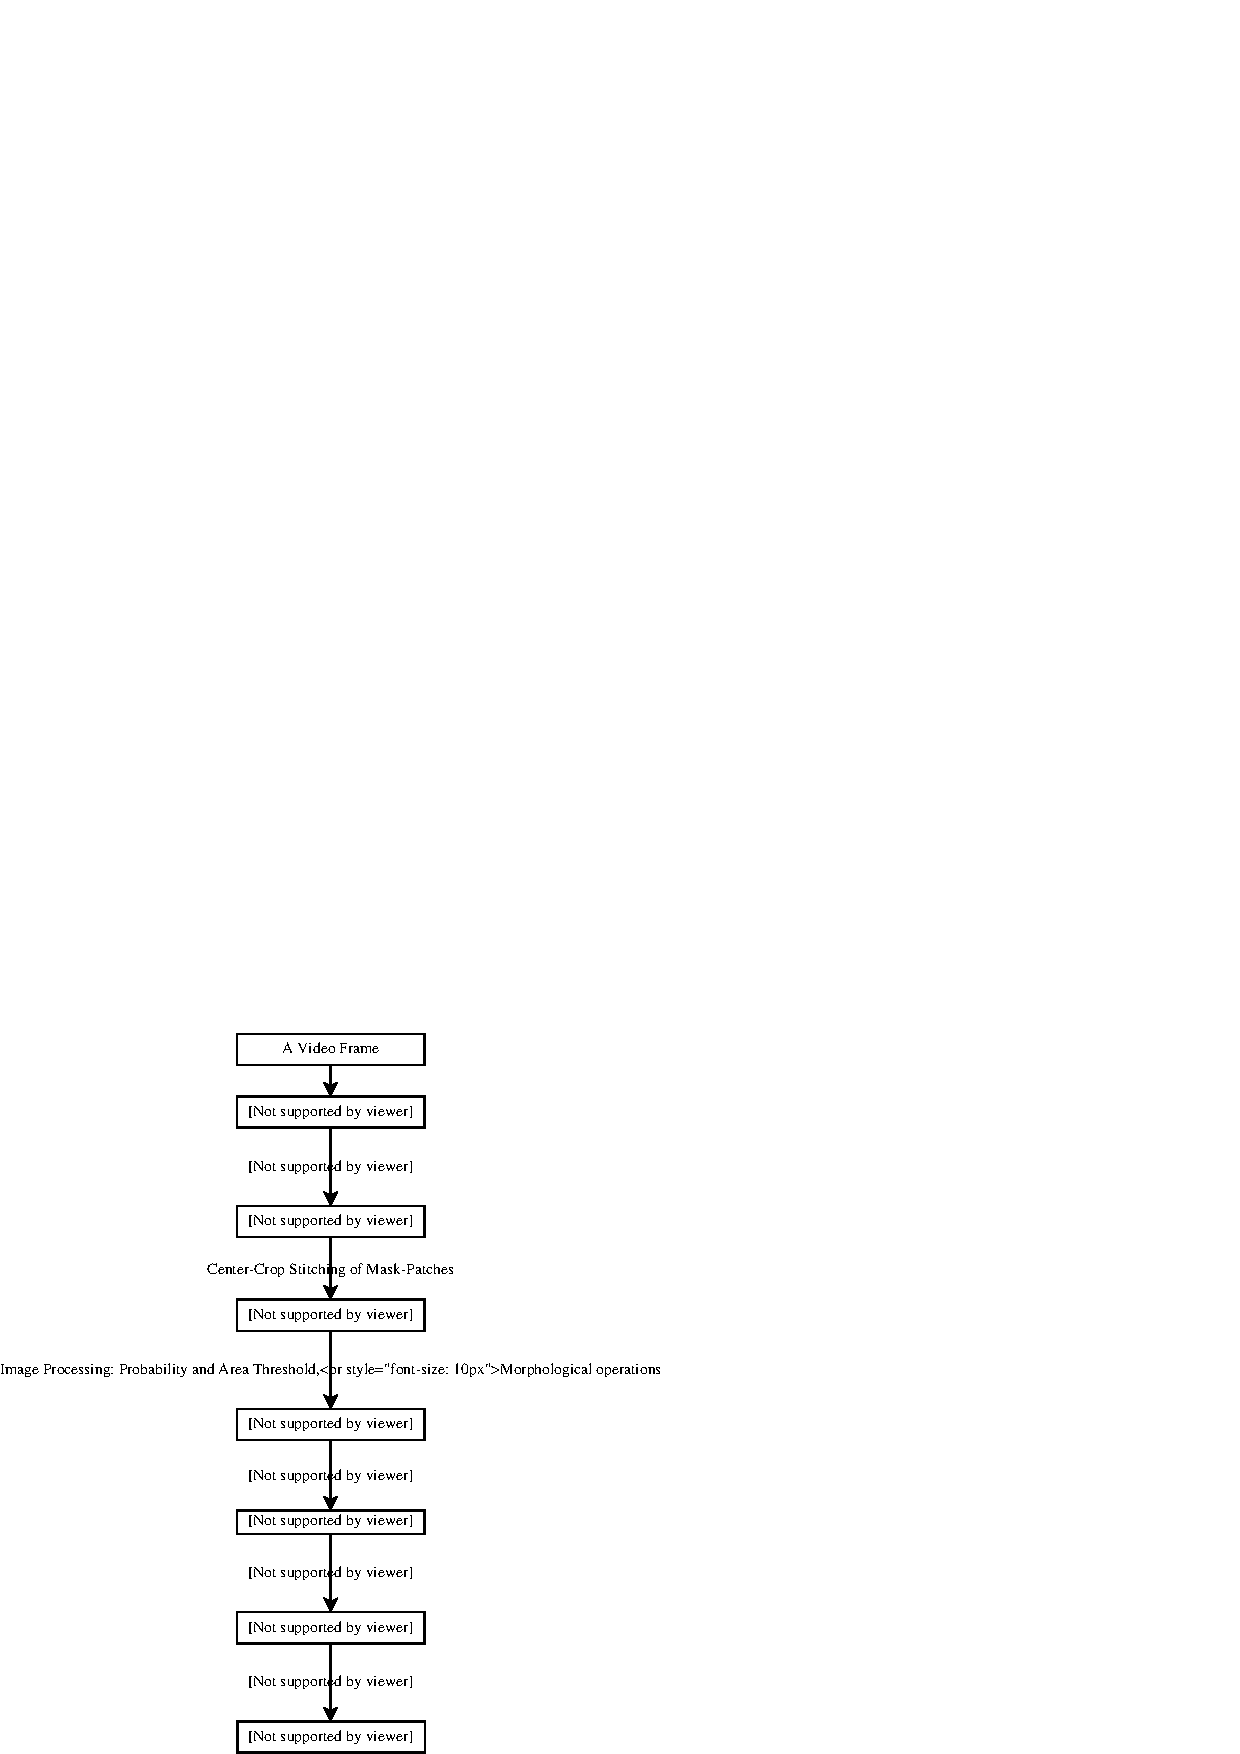
\includegraphics[width=0.8\linewidth]{flowchart.pdf}
\end{center}
   \caption{Flowchart depicting the joint UNet-VGG16 inference pipeline.}
\label{fig:long}
\label{fig:flowchart}
\end{figure}

\subsubsection{Region Proposal using Semantic Segmentation}
Upon observation over several annotated masks, we selected a square patch-size 256 pixels on each side to be an appropriate, as it was sufficient to contain most of the scaleworms. Therefore, during the training time, a patch of 256x256 was extracted around every labeled scaleworm to form the train images, and the corresponding ground truth mask-patch (a 256x256 patch of the labeled scaleworm mask) was extracted around the labeled mask. Note that every train patch contained a scaleworm, and patches having no scaleworms (i.e., having empty patch-masks) were not included in UNet training as it works at a pixel-level. Relevant image augmentations (rotation, shear, height/width shift, zoom, flip) were used on the train data to increase the model robustness. The standard UNet architecture \cite{unet} was modified to include a batch-normalization layer after every convolution layer to help in faster convergence and to add a regularizing effect \cite{batchnorm}. This modified UNet was trained with the patches to learn the corresponding mask-patches, to minimize a binary cross-entropy loss using Adam optimization algorithm with a learning rate of $10^{-3}$. Trial and error experiments were conducted to choose the learning rate which led to a faster convergence which also resulted in lower loss.
This model was trained for thousand epochs saving the model found across the epochs. % TODO: This line is too much implementation detail, which could be omitted.

During the inference time (as shown in Figure \ref{fig:flowchart}), the input video-frame was split into multiple patches of the size 256x256, using a sliding window which strides 128 pixels (half the patch-size). Such an overlapping strided-patches were chosen to ensure that we capture those scaleworms which could get split across different patches. Each strided patch was input to the trained UNet model, to get a predicted mask-patch which is a grey-scale mask indicating predicted probabilities. Such predicted mask-patches from all the strided patches from a video-frame were stitched back to form a single predicted mask using center-crop stitching as shown in Figure \ref{fig:centercropstitc}, to get a semantic segmentation mask of the video-frame.

\begin{figure}[t]
\begin{center}
   \includegraphics[width=0.8\linewidth]{center_crop_stitch.png}
\end{center}
   \caption{Center-Crop Stitch method to stitch strided (stride-length is half the patch-size) patches to form the whole image. The dotted and the solid squares (red) represent two subsequent patches of size 256x256. The squares shown for the center crop of each patch (green) are half the size of the patch (128x128), hence it aligns when concatenated in same order with the center crop of the subsequent patch. This helps in restoring the predicted mask of a scaleworm (pinkish worm at the center) which is split across strided patches.}
\label{fig:long}
\label{fig:centercropstitch}
\end{figure}

UNet \cite{unet} considers color and the structural information in the available context to predict whether or not a pixel belongs to the objects of interest. It often resulted in false-positives due to confounding color profiles. An additional post-processing step was added to the inference pipeline to perform simple image processing operations on the semantic segmentation masks to reduce the false positives. For instance, probability threshold was applied to consider only those pixels which have been predicted with high probability, and area threshold was applied to remove connected-components which were larger or smaller than empirically set upper and lower bounds of allowed scaleworm sizes respectively. Also simple morphological operations like dilation can be applied. This flexibility helps to control the output of the UNet and helps in debugging as well, but these fixed operations could lead to non-generalizability. Therefore, we suggest that the post-processing of the semantic segmentation mask should be limited to simple and widely applicable operations. This results in the post-processed segmentation mask for the video-frame, where each connected-component is considered as a region proposal, which is a candidate for a valid scaleworm.

\subsubsection{Validation of Region Proposals}
We extract a 256x256 candidate patch from the original video-frame corresponding to each connected-component of the post-processed segmentation mask (found in the previous step), and input it to a binary classifier to determine whether this region proposal is a valid scaleworm or not. We consider the VGG-16 \cite{vgg16} classification architecture with minor modifications to reduce parameters in the dense layer which helps in limiting potential over-fitting due to less data in our case. Also, batch-normalization layers were included after every convolutional layer as it helps in early convergence and also due to its regularization effect \cite{batchnorm}.

Valid-scaleworm training samples were picked from The same strided patches that were used to train the UNet were used to form the valid-scaleworm (positive) training samples. For invalid-scaleworm (negative) training samples, we considered two types of data. First, we considered randomized set of patches which consisted of several randomly cropped patches from various video-frames where scaleworms are not present (manual verification was done to remove those random patches which included scaleworms). Second, we considered manually labeled patches which consisted of patches with non-scaleworm objects which lie in the areas where scaleworms are generally found, and which can be confused to scaleworms. Both valid and invalid scaleworm patches were used to train the VGG-16 binary classifier network, to minimize the cross-entropy loss using Adam optimization algorithm with learning rate $10^{-3}$. Relevant image augmentations (rotation, shear, height/width shift, zoom, flip) were used on the train data to increase the model robustness.

During inference time (refer to Figure \ref{fig:flowchart}), each 256x256 candidate patch is input to the trained VGG16 which predicts the probability of the candidate patch containing a valid-scaleworm. This predicted probability is used as a final score for each individually identified scaleworm, and the corresponding mask is picked from the post-processed mask. Further, a threshold is applied on this score to predict whether a region proposal is a valid-scaleworm or not. Finally, we get the count of valid-scaleworms in a video-frame, and their respective location and sizes from the mask.

%-------------------------------------------------------------------------
\section{Results and Discussion}
In this section, we briefly discuss the individual performances of UNet and VGG16 models, followed by a step-by-step result of the inference pipeline. Then, we discuss the overall instance segmentation performance evaluation using AP@[0.5] score (refer to section \ref{section:evalmethod}). Further, we discuss the impact on performance caused due to addition of data and retraining of certain parts of the architecture through 3 different experimental analyses.

\subsection{Individual Model Performance}
Data was collected in two different sets as described in \ref{section:data}. Set 1 (S1) contained $261$ training patches and corresponding labeled patch-masks, and set 2 (S2) contained $276$ training patches and patch-masks. Hence, two different UNet models were trained - version 1 (V1) with train data from S1, and version 2 (V2) with train data from S1 and S2 (total of $537$ patches). Each of these models converged to a high training and a very close validation accuracy indicating that it was not overfit on train data. The converged models produced a mean IoU of $0.926$ and $0.937$ respectively on the validation set.

Similarly, three different VGG16 models were trained - version 1 (V1) with train patches from S1, version 2 (V2) and version (V3) with train patches from S1 and S2. All VGG16 models (V1, V2 and V3) included $\approx 400$ \textit{randomly cropped negative patches} (patches that do not include a valid scaleworm). VGG16 model Version 3 (V3) was trained with an additional $\approx 1000$ \textit{Custom Negative (CN) patches which were manually labeled}, and these contained objects that could be confused to scaleworms. Each of these models converged to a validation accuracy close to $0.99$.

Therefore, the individual models were trained well without overfitting on the relatively small training data. We observed that addition of batch-normalization layers to both the models helped them in converging much faster than the original architecture without batch-normalization layers.

%- Batch norm efficacy. val_mean_iou vs number of epochs, for with batchnorm vs without bathcnorm. (should this be in results section? this kind of helped in making the decision for the methodology, so this can be in methodology also, right?)

\subsection{Inference Pipeline Experimental Results} \label{section:experiments}
One of each trained models of UNet and VGG16 can be plugged in the inference pipeline discussed in the section \ref{section:inferencepipeline}. Figure \ref{fig:inferenepipelineoutput} shows the intermediate results of the inference pipeline when UNet V2 and VGG16 V3 were used in the inference pipeline. We can observe that the final instance segmentation output is visually reasonable. This inference pipeline setting resulted in a AP@[0.5] of $0.671$.
%<flow of images in the pipeline to get the final output.> show the segmentations, but with overlay, its not really visible, so remove the overlay in the last image.

Now, we perform rigorous experimentation and evaluate the method using the AP@[0.5] metric. We perform the following three experiments whose results have been summarized in Table \ref{tab:results}.

- First, ... We observe that ...

- Seconds, ... We observe that ...

- Third, ... We observe that ...

\begin{table}[]
\caption{Results from the experiments of the proposed joint UNet-VGG16 inference pipeline as described in the section \ref{section:experiments}.}
\label{tab:results}
\begin{tabular}{|c|l|l|l|}
%\centering
\hline
\multicolumn{1}{|l|}{\textbf{Experiment}} & \textbf{UNet} & \textbf{VGG16}    & \textbf{AP@{[}0.5{]}} \\ \hline
\multirow{3}{*}{\textbf{Exp. 1}}          & V1 (S1)       & V1 (S1)           & 0.451                 \\ \cline{2-4} 
                                          & V2 (S1 + S2)  & V2 (S1 + S2)      & 0.563                 \\ \cline{2-4} 
                                          & V2 (S1 + S2)  & V3 (S1 + S2 + CN) & 0.671                 \\ \hline
\multicolumn{4}{|l|}{}                                                                                \\ \hline
\multirow{3}{*}{\textbf{Exp. 2}}          & V1 (S1)       & V1 (S1)           & 0.451                 \\ \cline{2-4} 
                                          & V1 (S1)       & V2 (S1 + S2)      & 0.556                 \\ \cline{2-4} 
                                          & V1 (S1)       & V3 (S1 + S2 + CN) & 0.589                 \\ \hline
\multicolumn{4}{|l|}{}                                                                                \\ \hline
\multirow{2}{*}{\textbf{Exp. 3.1}}        & V1 (S1)       & V1 (S1)           & 0.451                 \\ \cline{2-4} 
                                          & V2 (S1 + S2)  & V1 (S1)           & 0.487                 \\ \hline
\multirow{2}{*}{\textbf{Exp. 3.2}}        & V1 (S1)       & V2 (S1 + S2)      & 0.556                 \\ \cline{2-4} 
                                          & V2 (S1 + S2)  & V2 (S1 + S2)      & 0.563                 \\ \hline
\multirow{2}{*}{\textbf{Exp. 3.3}}        & V1 (S1)       & V3 (S1 + S2 + CN) & 0.589                 \\ \cline{2-4} 
                                          & V2 (S1 + S2)  & V3 (S1 + S2 + CN) & 0.671                 \\ \hline
\end{tabular}
\end{table}


- <table> with both unet+cnn trained on set1, set2, and set3. adding data helps in increasing the average precision. Therefore, we can spend more on getting the data to get better model.

- But this concerns maintainability, since we have to train two different models. Understand the imnprovement in average precision by just CNN or Just UNet. 

- <table> Keep v0.4 UNet constant, and keep adding data and training CNN. We observe a great increment. So CNN model contribues a lot.

- <table> What if we consider UNet trained on very less data, i.e., set 1. Still CNN keeps increasing the accuracy, but after some point it tends to not lead to high increase in accuracy. At that time, we might want to update UNet model.

- <table> show that keeping CNN model constant, improvement in UNet did not improve in any accuracy. This is mainly the case, because our final score mainly depends on CNN. (So this table might not be very useful)

-<training time on dataset of x size with batchsize, and inference time on an image>

\subsection{Advantages}

- Easy to debug and fix the model and work with limited labeled data which is essential when such data cant be crowdsourced for labeling.

- Sparse labeling is important because its hard to tag each and every scaleworm.

<Image showing where it is still not working>
- Can be overcome by iteratively identifying and all new negative patches. And thats how we can debug and control the model.

- Sparse labeling will suffice.

- Worked on relatively less data compared to the requirement of other Models which were not feasible with such low amount of data. (Hard to claim this. So we can try to put a reference showing that Other models need a lot of data.)

- Training and Testing since done on small patches, it can fit in personal computer GPU's like GTX 970. And relativels runs fast because of less parameters.

\subsection{Disadvantages}
- The score doesn't quantify the errors from UNet. Since CNN is the main contribution for getting the improvement, it is ok. But if we wanted Average recall, then we would need to propagate errors from UNet as well.

- We had a relatively small test set. Results from larger test sets could be useful. But hard to get more dense labeling for testing purpose.

%-------------------------------------------------------------------------
\section{Conclusion and Future Work}

This provides a decent result with a fairly simple model to start getting structures metadata info like count scaleworms, and the size of each scaleworm, in each of the scenes for a video. it is easy to debug and understand what kind of data needs to be added to improve it, and therefore by adding more data it has proven to improve, and especially by adding specific datam, it would improve in a larger magnitude. If run on all the data, we get a temporal distribution of scaleworm population, which could be very useful dataset to perform population study espectially by comparing the with the temperature at the hydrothermal vent to understand their behavior.

Future work may consider trying other more complex models on the data. MaskRCNN, PaNet could be tried. If segmentation is not required not, SSD, FasterRCNN can be tried on this data. The temporal information in the video, can also be exploited to identify the scaleworms with higher precision, as other objects would occilate but scaleworm wouldn't be oscillating in a short video-segment.

This prototype could help in adopting such techniques to such many other different organisms, some of which pose more challenges, and could help benthic biologists explore more of this hidden world of rich and diverse ecosystem near hydrothermal vents.

%-------------------------------------------------------------------------

{\small
\bibliographystyle{ieee}
\bibliography{egbib}
}


\end{document}
